\documentclass{standalone}
\usepackage{tikz}
\usepackage{siunitx}
\usepackage{mathtools}
\usepackage[dutch]{babel}
\usepackage{mathpazo}
\usepackage{microtype}
\usetikzlibrary{positioning,arrows.meta,backgrounds}
\definecolor{uablue}{RGB}{0,61,100}
\colorlet{uablue25}{uablue!25}
\definecolor{uared}{RGB}{126,0,47}
\colorlet{uared25}{uared!25}
\definecolor{uagreen}{RGB}{0,126,1}
\colorlet{uagreen25}{uagreen!25}
\tikzset{input_variable/.style={circle,draw=uablue,fill=uablue25}}
\tikzset{%
    oppervlakte/.pic={%
        \useasboundingbox node[input_variable] {};
        \draw (0,0) -- (.75,0) node[midway,input_variable] {};
    }
}
\newcommand{\doorstreken}[2][]{%
    \draw[#1,uablue] (#2) -- +(-1,0) -- +(1,0)
}
\begin{document}
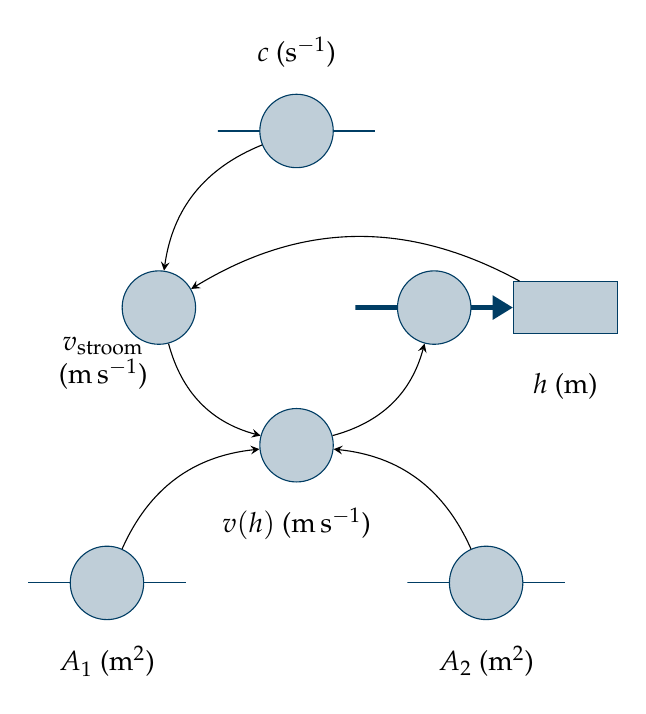
\begin{tikzpicture}[auto]
    \begin{scope}[inner sep=2ex,node distance=15ex,every node/.style={input_variable}]
        \node[] (vh) {};
        \node[below left of=vh,xshift=-4ex] (a1) {};
        \node[below right of=vh,xshift=4ex] (a2) {};
        \node[above left of=vh] (v) {};
        \node[above right of=v,yshift=3ex] (c) {};
        \node[above right of=vh] (x) {};
    \end{scope}
           %%% 
    \begin{scope}[on background layer]
        \doorstreken{a1};
        \doorstreken{a2};
        \doorstreken{c};
        \doorstreken[->,>=Triangle,ultra thick]{x} coordinate (Z);
    \end{scope}
    \node[anchor=west,draw,rectangle,inner sep=2ex,minimum width=8ex,uablue,fill=uablue25] (h) at (Z) {};
    %%%%
        \node[below of=a1] {$A_1$ (\si{\meter\squared})};
        \node[below of=vh] {$v(h)$ (\si{\meter\per\second})};
        \node[below of=a2] {$A_2$ (\si{\meter\squared})};
        \node[above of=c] {$c$ (\si{\per\second})};
        \node[below of=h] {$h$ (\si{\meter})};
        \node[below left of=v,align=center] {$v_{\text{stroom}}$\\(\si{\meter\per\second})};
    \path[>=stealth,->]
        (h) edge[bend right] (v)
        (c) edge[bend right] (v)
        (a1) edge[bend left] (vh)
        (a2) edge[bend right] (vh)
        (vh) edge[bend right] (x)
        (v) edge[bend right] (vh)
        ;
\end{tikzpicture}

\end{document}
